\chapter{Genome assembly and characterization}
\section{Introduction}
Ascidians are marine invertebrates that spend their adult life filter feeding through an incurrent siphon and an outcurrent siphon. Ascidians are evolutionarily interesting because of the phylogenetic position -- they are tunicates, the sister group to vertebrates and cephalochordates, with whom they form the chordate phylum. Although ascidians share little morphological resemblance to vertebrates in their adult stage, they do share several features in their larval stage: a notochord, dorsal hollow neural tube, and gill slits during development \cite{wada_details_1994,cameron_evolution_2000}. 

The development of ascidians is well documented, and the cell lineage from fertilization to gastrulation has been described thoroughly in \textit{Ciona intestinalis} \cite{nishida_cell_1983,nishida_cell_1985,nishida_cell_1987}. Studies of other ascidian species have shown that the majority of the phyla members have an invariant cell lineage and typical development \cite{berrill_studies_1931}. However, a few solitary ascidians have deviated from the typical developmental program and undergone tail-loss \cite{swalla_interspecific_1990, tsagkogeorga_updated_2009}. \textit{M. occulta} and \textit{M. oculata} are two species that are found in the shallow waters for Roscoff, France that closely resemble each other-- in their adult stage, they differ only by a white pigment spot found between the siphons of \textit{M. oculata} (Figure~\ref{fig:adults}). These two \textit{Molgula} species, however, have different methods of development\textemdash \textit{M. oculata} develops as a typical tadpole larvae and \textit{M. occulta} develops without a tail. The underlying molecular reasons for divergence are unknown.

Many ascidian genes have been studied across a number of ascidians, showing that gene function tends to be orthologous within the phyla \cite{satoh_ascidian_2003}. Although genes tend to be expressed in homologous patterns and tissues, the presence of genes are not the same across species. There are a number of cases where a gene that has been shown to be necessary for a phenotype in one species is completely absent in other ascidian species with the same phenotype \cite{lemaire_ascidians_2008}. Ascidian species are far more divergent than they appear phenotypically. It has been shown that in ascidians with the same phenotype and gene expression, regulatory modules are not necessarily the same \cite{hudson_divergent_2011,kugler_evolutionary_2011,stolfi_divergent_2014}. This is often attributed to the conservation of gene regulatory networks (GRNs) and the flexibility of TF binding site distribution in a given enhancer, which contribute to conservation of enhancer function \cite{hare_careful_2008}. This regulatory turnover is termed ?developmental system/systems drift? (DSD) (True and Haag, 2001). This term broadly applies to the divergence in the molecular or morphogenetic basis for the development of identical homologous characters. 

Tunicates have even deviated from \textit{hox} patterning and function \cite{ikuta_limited_2010}, and here genomics has shed some light on the area. Ascidians are broadcast spawners, which leads to them being highly polymorphic and having rapid rates of evolution \cite{dehal_draft_2002}. This drives rapid divergence in genomes outside of coding regions, as well as change of gene function when compared to other chordates \cite{lemaire_ascidians_2008}. %We will demonstrate this divergence using two closely related species \textit{M. occulta} and \textit{M. oculata}, and the more divergent \textit{M. occidentalis}. 
Through whole genome sequencing and assembly of two closely related species \textit{M. occulta} and \textit{M. oculata}, and the more divergent \textit{M. occidentalis}, we have %given us a better picture of what is going on evolutionarily for both close and divergent species, and allows us to characterize gene networks, identify regulatory elements and gain better understanding of the mechanisms driving conserved development in ascidians.
demonstrated that \textit{M. occidentalis}, \textit{M. occulta}, and \textit{M. oculata} all have different \textit{hox} configurations, and while having invariant development, the cis-regulatory elements behind the development has diverged between \textit{Ciona} and \textit{Molgula}.

\begin{figure}[tbp]
\centering
\includegraphics[scale=0.5]{figures/adults.pdf}
\caption{\textbf{Adult ascidians.} \textit{M. occulta} (A) and \textit{M. oculata} (B) are nearly identical in their adult stage with the white pigment spot (red arrow). Their tunic is covered in sand, since they are found on the sandy sea bottoms. Under their sand covered tunic, the two species differ by the color of their eggs\textemdash purple in \textit{M. oculata}, pictured, and an orange-yellowish color in \textit{M. occulta}\textemdash which are found just above the kidney complex (C). \textit{C. intestinalis} (D) is the best studied ascidian and has a well-assembled and annotated genome.}
\label{fig:adults}
\end{figure}

\section{Materials and methods}

\subsection{Genomic DNA library preparation and sequencing}
Genomic DNA was phenol/chloroform extracted from dissected gonads of \textit{Molgula occulta} (Kupffer) and \textit{Molgula oculata} (Forbes) adults from Roscoff, France, and a \textit{Molgula occidentalis} (Traustedt) adult from Panacea, Florida, USA (Gulf Specimen Marine Lab). Genomic DNA was sheared using an M220 Focused-ultrasonicator (Covaris, Woburn, MA). Sequencing libraries were prepared using KAPA HiFi Library Preparation Kit (KAPA Biosystems, Wilmington, MA) indexed with DNA barcoded adapters (BioO, Austin, TX). Size selection was performed using Agencourt (Beckman-Coulter, Brea, CA) AMPure XP purification beads (300-400 bp fragments), or Sage Science (Beverly, MA) Pippin Prep (650-750 bp and 875-975 bp fragments). For \textit{M. occulta} and \textit{M. occidentalis} libraries, 6 PCR cycles were used. For \textit{M. oculata} libraries, 8 cycles were used for the 300-400 bp library, and 10 cycles were used for the 650-750 and 875-975 bp libraries. Libraries of different species but same insert size ranges were multiplexed for sequencing in three 2x100 PE lanes on a HiSeq 2000 sequencing system (Illumina, San Diego, CA) at the Genomics Sequencing Core Facility, Center for Genomics and Systems Biology at New York University (New York, NY). Thus, each lane was dedicated to a mix of species, specifically barcoded libraries of a given insert size range. Raw sequencing reads were deposited as a BioProject at NCBI under the ID\# PRJNA253689.
\subsection{Genome sequence assembly}
All genomes were assembled on Michigan State University High Performance Computing Cluster (\url{http://contact.icer.msu.edu}). Prior to assembly, read quality was examined using FastQC v0.10.1. Reads were then quality trimmed on both the 5' and 3' end using seqtk trimfq (\url{https://github.com/lh3/seqtk}) which uses Phred algorithm to determine the quality of a given base pair. Seqtk trimfq only trims bases, so no reads were discarded. Each library per species was then abundance filtered using 3-pass digital normalization to remove repetitive and erroneous reads \cite{brown_reference-free_2012,schwarz_genome_2013,howe_tackling_2014}. Genome assembly was done using velvet v1.2.08 \cite{zerbino_velvet:_2008} with k-mer overlap length (`k') ranging from 19 to 69 and scaffolding was done by Velvet, by default. Velvet does not produce separate files for contigs and scaffolds; because Velvet scaffolded conservatively, contigs dominated the assemblies so we refer to both contigs and scaffolds as contigs. CEGMA scores were then computed to evaluate genome completeness \cite{parra_cegma:_2007}. The latest versions of three species' genome assemblies have been deposited on the ANISEED (Ascidian Network for In Situ Expression and Embryological Data) database for browsing and BLAST searching at http://www.aniseed.cnrs.fr/ \cite{tassy_aniseed_2010}. Scripts for genome assembly and CEGMA analysis can be found in the following github repository: \url{https://github.com/elijahlowe/molgula_genome_assemblies.git}
\subsection{Gene identification and alignments}
Thirty-nine hox genes were identified in human and downloaded from the NCBI database. These sequences were then BLASTed against each of the three assembled \textit{Molgula} genomes. The alignments were then extracted and BLASTed against the NCBI non-redundant database. \textit{Molgula} aligning sequences were extracted, annotated and placed in the following files, mocc\_hox\_aa.fa, mocu\_hox\_aa.fa, and moxi\_hox\_aa.fa, which are located at \url{https://github.com/elijahlowe/eli_last_rodeo-/data}. \textit{Hox1-13} sequences for human, fruit fly, and Amphioxus were download from `Homeobox Database' (http://homeodb.zoo.ox.ac.uk/). These sequences were then joined in a multifasta file with the identified Molgula \textit{hox} genes and used to produce a phylogenetic trees using MAFFT version 7 online rough tree program at \url{http://mafft.cbrc.jp/alignment/server/clustering.html} \cite{katoh_parttree:_2007,katoh_mafft_2013}.  Additional alignments between the three species were conducted using mVista \cite{mayor_vista_2000,frazer_vista:_2004,visel_vista_2007} with \textit{M. oculata} as the anchoring sequence because it shows the most similarity between the three \textit{Molgula} species. The LAGAN alignment algorithm was used with translated anchoring to improve alignment because of evolutionary distances\cite{brudno_lagan_2003}.    

\section{Results}
\subsection{Genome assemblies assessment}
Genomes of three Molgula species (\textit{M. occidentalis}, \textit{M. oculata}, and \textit{M. occulta}) were sequenced using next-generation sequencing technology and assembled. A common metric for judging the quality of a genome assembly is the contig N50 length, which is determined such that 50\% of the assembly is contained in contigs of this length or greater. We used the contig N50 length to select the best assembly for each species given the varying `k' parameter (length of k-mer overlap). A `k' of 39 yields the best assembly for both \textit{M. occidentalis} and \textit{M. occulta}. The best `k' for \textit{M. oculata} was 61. \textit{M. occidentalis}, \textit{M. occulta}, and \textit{M. oculata} N50 lengths were approximately 26.3 kb, 13 kb, and 34 kb, respectively (Table~\ref{table:genome_table}).

\begin{table}[tbp]
\centering
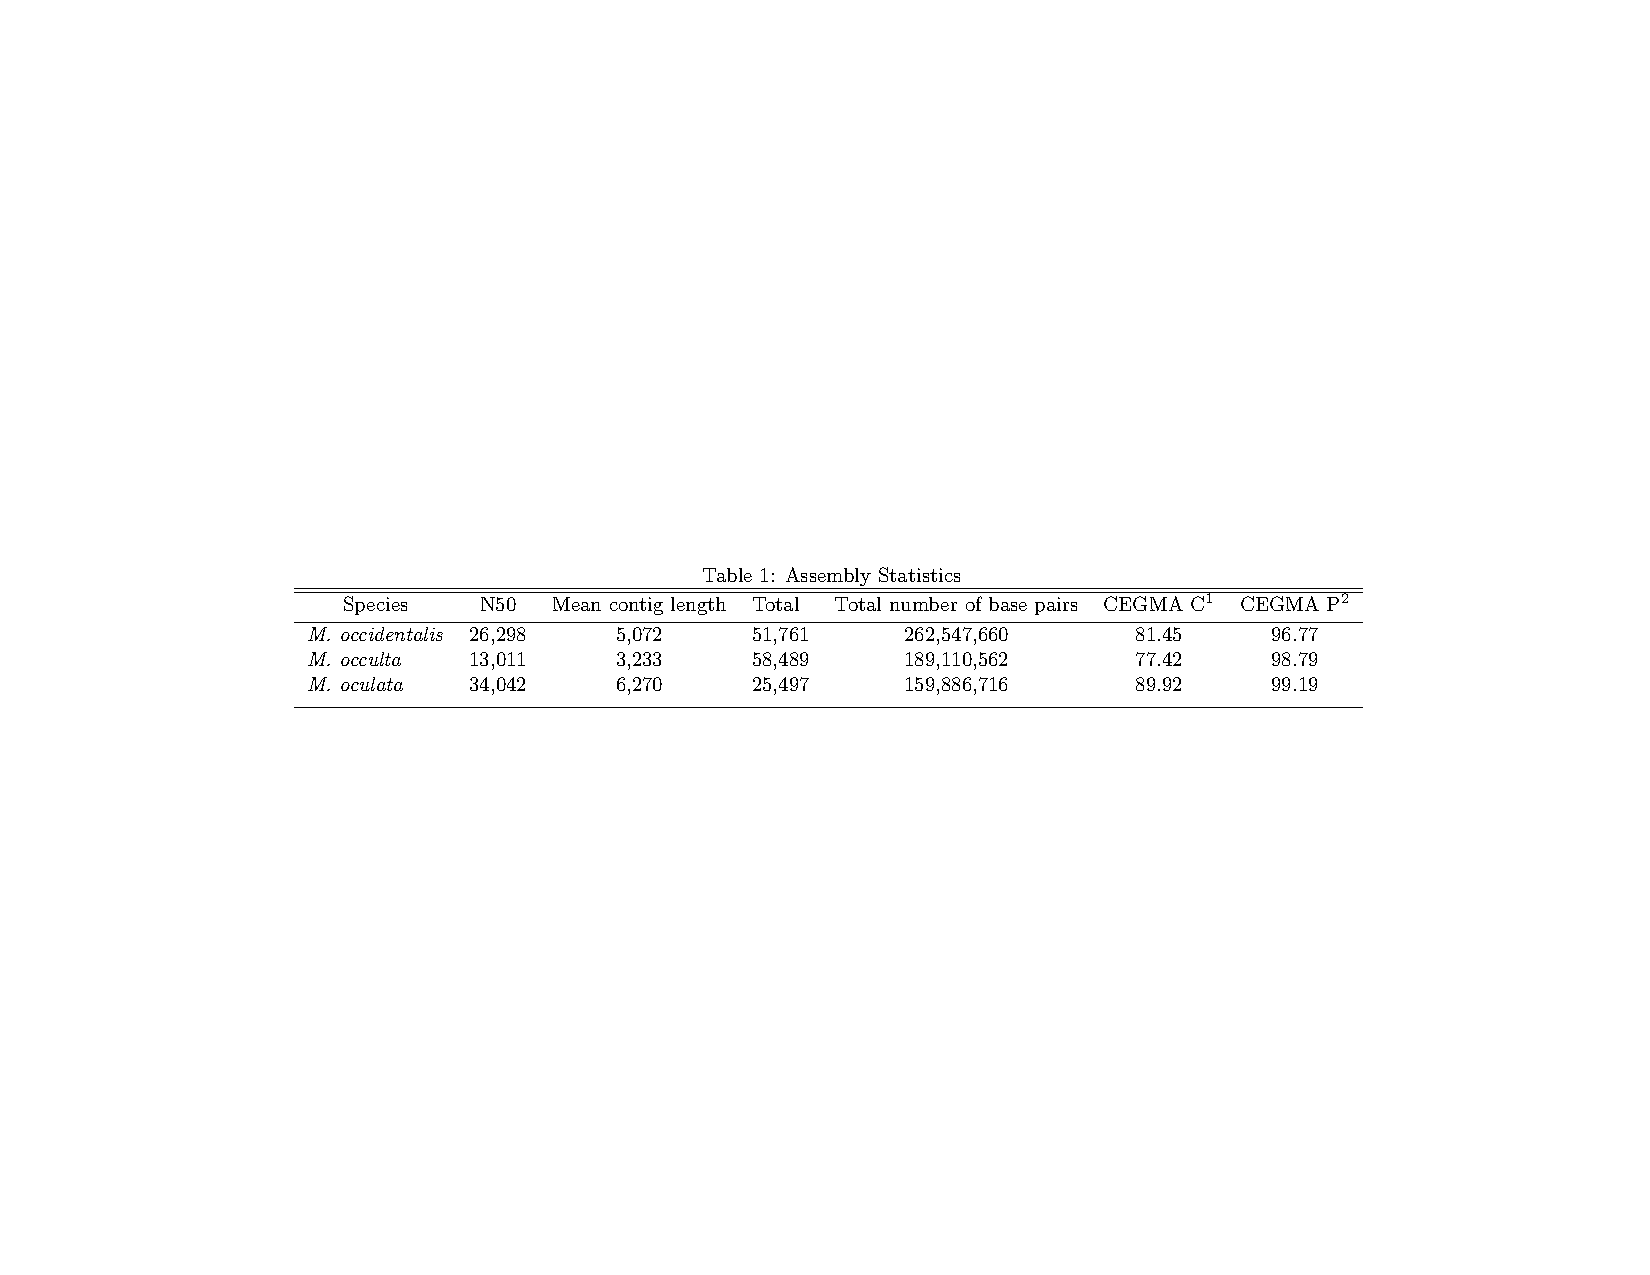
\includegraphics[width=\linewidth]{figures/genome_table_1}
\caption{\textbf{Genome assembly statistics.} The contig N50 length, mean contig length, total number of contigs, total number of base pairs and CEGMA scores were collected for each draft assembly. The CEGMA score is a metric of completeness measured against highly conserved eukaryotic genes. Alignments of 70\% or greater of the protein length are called complete (C) and all other statistically significant alignments are called partial (P).}
\label{table:genome_table}
\end{table}

In addition to N50 lengths, we also used CEGMA (Core Eukaryotic Genes Mapping Approach) scores, in order to evaluate the assemblies' representative completeness \cite{parra_cegma:_2007}. CEGMA reports scores for complete and partial alignments to a subset of core eukaryotic genes. An alignment is considered ``complete'' if at least 70\% of a given protein model aligns to a contig in the assembly, while a partial alignment indicates that a statistically significant portion of the protein model aligns. The partial alignment scores are \mytilde97\% or higher for all assemblies. \textit{M. oculata} has the best complete alignment score at \mytilde90\%. \textit{M. occidentalis} and \textit{M. occulta} have complete alignment scores of 81\% and 77\% respectively (Table~\ref{table:genome_table}). These scores indicate that our assemblies contain at least partial sequences for the vast majority of protein-coding genes in the genomes of these species.
Various factors make it unreliable to predict genome size and gene density based on assembly metrics alone \cite{bradnam_assemblathon_2013}. Of the handful of sequences we isolated and analyzed, we found that the sizes of introns and upstream regulatory regions were roughly comparable to those from their \textit{Ciona} orthologs. This suggests that the \textit{Molgula} genomes may be as compact as the \textit{C. intestinalis} genome (i.e., \mytilde150-170 Mb, \mytilde16,000 genes) \cite{laird_chromatid_1971,simmen_gene_1998,satou_improved_2008}.

\subsection{Gene complexes}
\textit{Hox} genes are a subset of the homeobox genes and are known to be involved with the establishment of morphological identities along the anteroposterior axis of bilaterians and cnidarians \cite{finnerty_origins_2003}. All \textit{hox} genes have a highly conserved 60 amino acid (aa) homeobox sequence \cite{mcginnis_homologous_1984,gehring_homeodomain-dna_1994} and \textit{hox} genes are distinguished by variation of the homeobox domain. There are 4 \textit{HOX} clusters in humans totaling in 39 genes. Within tunicates, \textit{C. intestinalis}, \textit{Halocythia roretzi} and \textit{Oikopleura dioica} \textit{hox} genes have been characterized. \textit{C. intestinalis} has 9 \textit{hox} genes, \textit{Hox1} through \textit{6}, \textit{Hox10}, and \textit{Hox12-13} \cite{dehal_draft_2002}. The \textit{hox} gene of \textit{C. intestinalis} were initially found on 5 scaffolds spanning \mytilde{980} kb using the draft assembly, with \textit{hox2-4}, \textit{hox5-6} and \textit{hox12-13} being found on the same scaffold and later identified to be two clusters of \textit{hox} genes across two chromosomes \cite{ikuta_ciona_2004}. \textit{O. dioica} also has 9 \textit{hox} genes, \textit{hox1-2, hox4}, a duplicate \textit{hox9}, and \textit{hox10-13}, however, none of the genes have been found on the same scaffold, even using a 250 kb window \cite{siok_biological_2004}. 

Eight \textit{hox} genes have be found in \textit{M. occulta} and \textit{M. oculata}, while nine have been found in \textit{M. occidentalis}. The eight found were \textit{Hox1}, \textit{hox2}, \textit{hox3-4}, \textit{hox5}, \textit{hox10} and \textit{hox12-13}, with \textit{hox3} and \textit{hox 4} being found on the same contig in all three species (Figure~\ref{fig:hoxcluster}). Additionally \textit{hox10}, and \textit{hox12-13} are found on the same contig in \textit{M. oculata} with only \textit{hox12-13} being found on the same contig in \textit{M. occidentalis}. However, it appears that the \textit{hox} genes have been rearranged in \textit{M. oculata}, since \textit{hox10} is downstream of \textit{hox12-13}.  \textit{M. occidentalis} had one additional \textit{hox} gene compared to \textit{M. occulta} and \textit{M. oculata}, a duplicate \textit{hox10} gene \mytilde12kb apart found on the same contig. Also, the \textit{M. occidentalis} \textit{hox2} has a stop codon located in the 3-4 helix, although this may be specific to the animal examined and not the total population. The second \textit{hox10} sequence was not fully sequenced, missing 14 aa of the homeobox domain, and the identity of the two sequences was 52.1\% at a nucleotide level, 53.4\% at a protein level, and 91.3\% identical within the homeobox domain (Figure~\ref{fig:occihox10}). \textit{M. occulta}, \textit{M. oculata}, and \textit{M. occidentalis hox} genes span across 7, 5 and 6 contigs respectively and are 197 kb, 311.7 kb and 279 kb in length, respectively.  This is more compact than the \textit{Ciona} \textit{hox} cluster which exhibits longer than usual intergenic regions, averaging in the 5Mb range, when typically the \textit{hox} genes have 100-120 kb intergenic regions separating them \cite{mcginnis_homeobox_1992}. The \textit{hox} gene in the \textit{Molgula} had far smaller intergenic regions, 10-25 kb in length for the \textit{hox} genes that were found on the same contigs.  

\begin{figure}[tbp]
\centering
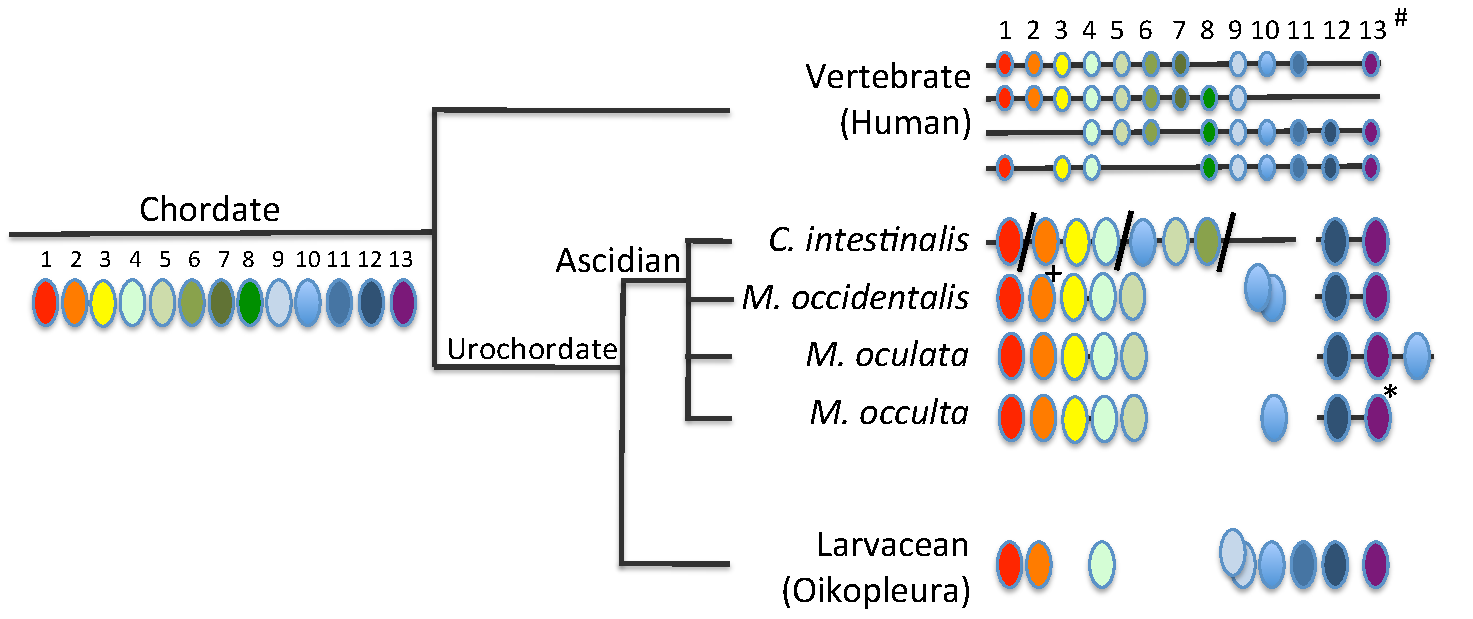
\includegraphics[scale=0.65]{figures/hox.pdf}
\caption{\textbf{Hox clusters for \textit{M. occulta}, \textit{M. oculata} and \textit{M. occidentalis}} Eight \textit{hox} genes were found in  \textit{M. occulta} and \textit{M. oculata}, while nine were found in \textit{M. occidentalis}. \textit{Hox1}, \textit{hox2}, \textit{hox3-4}, \textit{hox5}, \textit{hox10} and \textit{hox12-13} were found in all three \textit{Molgula} species. \textit{Hox3-4} was found on the same contig in all species, with \textit{hox12-13} found on the same contig in \textit{M. occidentalis} and \textit{M. oculata}. *\textit{M. occulta} \textit{hox12-13} is not found on the same contig, but when aligned using mVista, there is high sequence similarity, showing the possible placement of \textit{hox12-13} in \textit{M. occulta}. \textsuperscript{+}\textit{M. occidentalis} \textit{hox2} gene had a stop codon found in the 3-4 helix. \textsuperscript{\#} numbers correspond to gene color, and rearrangements have been found in \textit{Ciona} and \textit{Molgula}.}
\label{fig:hoxcluster}
\end{figure}

\subsection[title]{Divergence of GRN\footnote{Portions of this section was published in Stolfi et al., \cite{stolfi_guidelines_2014}.}}
Our sequencing efforts revealed extreme genetic divergence not only between \textit{Ciona} and \textit{Molgula}, as expected, but even within the Molgulids. For example, in Stolfi et al., \cite{stolfi_divergent_2014} we used BLAST to identify the \textit{Molgula} orthologs of \textit{C. intestinalis Mesp}. %(\textit{Ciinte.Mesp}, as per the proposed tunicate gene nomenclature rules, see Stolfi et al., \cite{stolfi_guidelines_2014}). 
\textit{C. intestinalis Mesp} is the sole ortholog of vertebrate genes coding for \textit{MesP} and \textit{Mesogenin bHLH} transcription factor family members \cite{satou_improved_2008}. VISTA alignment shows high sequence similarity between sequences 5' upstream of the \textit{Mesp} genes from the closely related \textit{M. oculata} and \textit{M. occulta}. However, there is no conservation of \textit{Mesp} DNA sequences, coding or non-coding, between \textit{M. oculata}/\textit{occulta} and \textit{M. occidentalis}, nor between \textit{C. intestinalis} and any of the three \textit{Molgula} species. In previous phylogenetic surveys, \textit{M. occidentalis} has been placed as an early-branching \textit{Molgula} species, often grouped together in a subfamily with species ascribed to the genera Eugyra and Bostrichobranchus instead \cite{hadfield_multiple_1995,huber_evolution_2000,tsagkogeorga_updated_2009}. Our sequencing results support the view that \textit{M. occidentalis} is highly diverged from other \textit{Molgula} species.

This sequence divergence is also evident when analyzing the \textit{hox} genes. When comparing sequence similarity of the \textit{hox} genes that were found on the same contigs (\textit{hox3-4} and \textit{hox12-13}), only regions clustered around the coding region for \textit{M. occulta} when compared to \textit{M. oculata} showed similarity, and only coding sequences showed similarity in \textit{M. occidentalis} when compared \textit{M. oculata} (Figure~\ref{fig:hox12}). This sequence similarity was a lot less obvious when comparing \textit{M. occulta} to \textit{M. occidentalis}. However, because of a lack of synteny outside of coding regions between \textit{M. occidentalis} and \textit{M. oculata} we were able to identify \textit{distal-less}, downstream of \textit{Hox13}, which is expressed in endodermal strand cells in \textit{Ciona}.

\begin{figure}[tbp!]
\centering
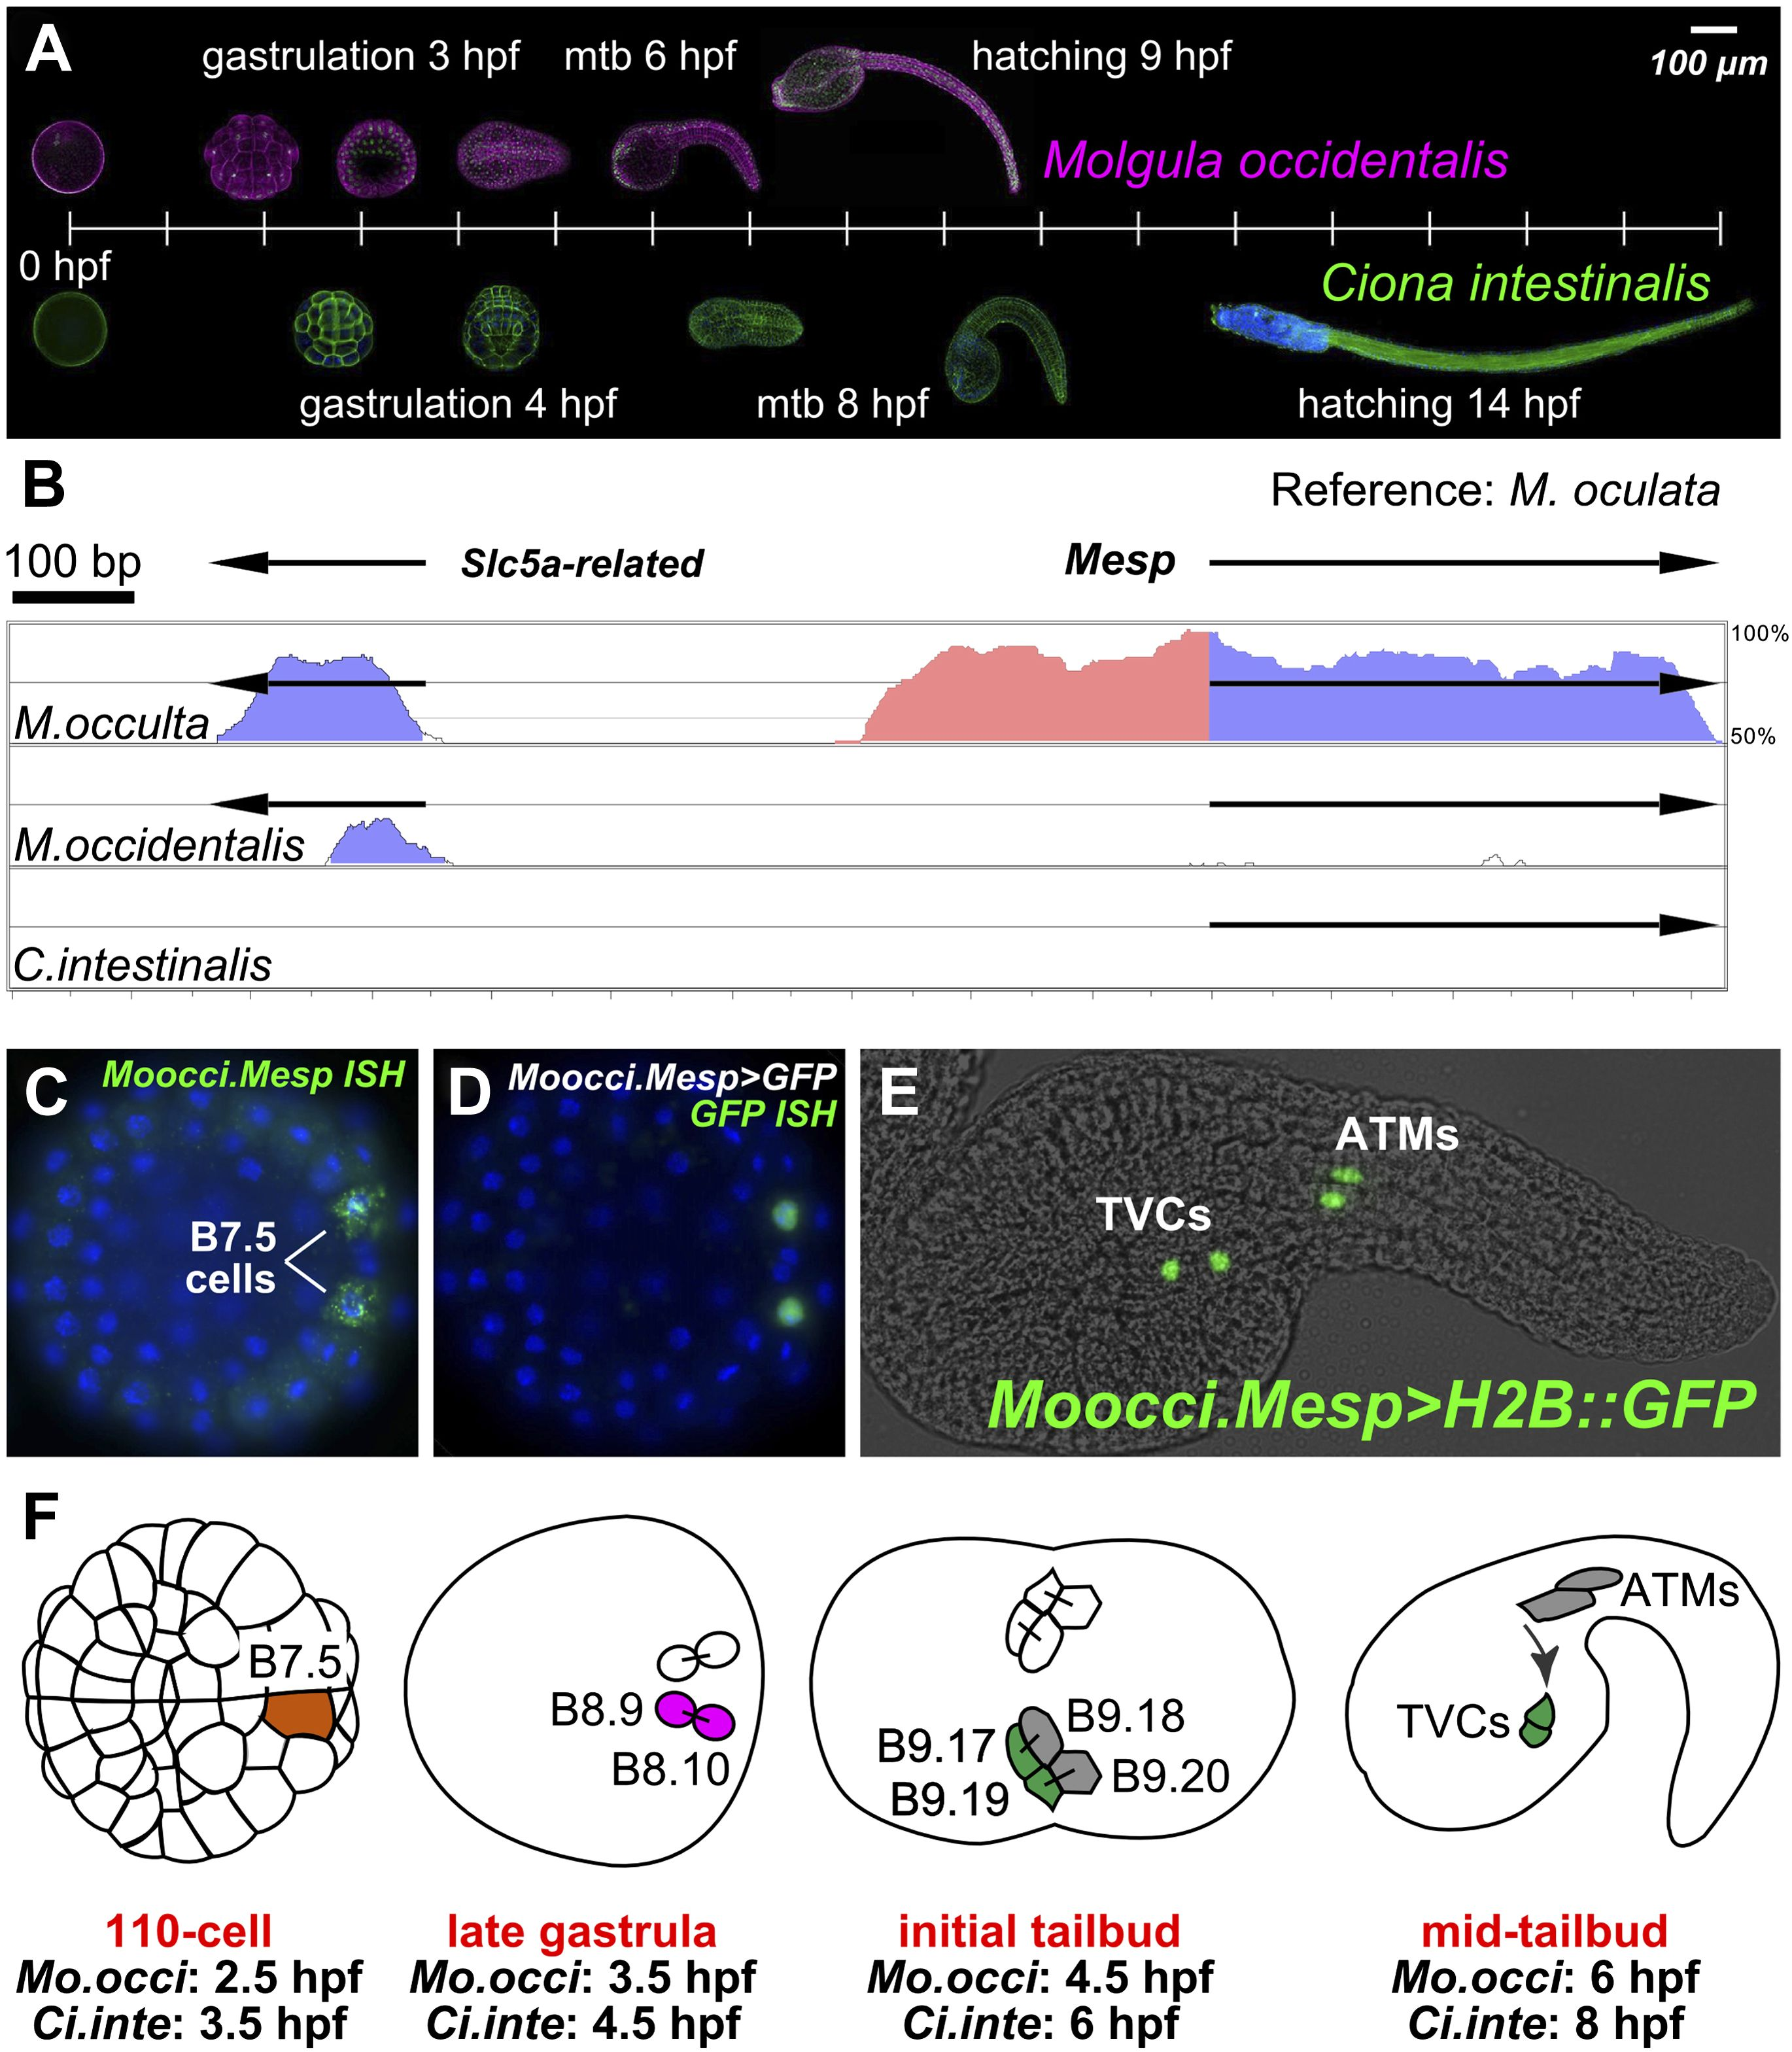
\includegraphics[scale=0.6]{figures/F1_large.jpg}
\caption{\textbf{The B7.5 lineage in \textit{M. occidentalis}} (A) Diagram comparing \textit{M. occidentalis} (top) and \textit{C. intestinalis} (bottom) embryogenesis at 24�C. Embryos were stained with Alexa Fluor dye-conjugated phalloidin to visualize cell outlines and DAPI to visualize cell nuclei. (B) Diagram of mVISTA (\cite{frazer_vista:_2004}; genome.lbl.gov/vista/) alignment of \textit{M. oculata Mesp (Moocul.Mesp)} locus to orthologs in \textit{M. occulta}, \textit{M. occidentalis}, and \textit{C. intestinalis}. Shaded peaks indicate sequence conservation above 70\% over 100-bp windows (blue = protein-coding, pink = non-coding). Arrows indicate direction of transcription of protein-coding genes. Non-coding sequences upstream of \textit{Mesp} are only conserved between \textit{M. oculata} and \textit{M. occulta}. \textit{M. occidentalis} and \textit{C. intestinalis} show considerable divergence even in protein-coding sequences. Note that microsynteny with SLC5A-related gene supports the orthology of these sequences among the Molgulids.}
\label{fig:mesp}
\end{figure}
\addtocounter{figure}{-1}
\begin{figure}[t]
  \caption{(C) In situ hybridization (ISH) for \textit{Moocci.Mesp} in 110-cell stage embryo (vegetal view), showing mRNA detection (green) in B7.5 blastomeres. Nuclei were counterstained with DAPI (blue). Staging is given by hours post-fertilization (hpf). (D) Vegetal view of a 110-cell stage embryo electoporated with \textit{Moocci.Mesp}>GFP reporter construct. Reporter gene expression was detected by ISH for GFP transcripts (green). Nuclei were stained with DAPI (blue). (E) Lateral view of a mid-tailbud stage embryo electroporated with Moocci. Mesp$>$Histone2B::GFP reporter construct. GFP fluorescence reveals B7.5 descendants on left side of embryo: two trunk ventral cells (TVCs) and two anterior tail muscles (ATMs). (F) Diagram of B7.5 lineage divisions from 110-cell stage to mid-tailbud stage, inferred from previous C. intestinalis studies. Cells are named according to Conklin's method (Conklin, 1905). The lineage is bilaterally symmetric, but only cells on the left side are indicated and named. Relative staging given for \textit{M. occidentalis (Mo.occi)} and \textit{C. intestinalis (Ci.inte)}. 110-cell and late gastrula: vegetal view. Initial tailbud: dorsal view. Mid-tailbud: lateral view. Anterior pole is on the left in all images and illustrations.
DOI: 10.7554/eLife.03728.003}% Continued caption
\end{figure}

\section{Expression of the \textit{M. occidentalis Mesp} gene marks the B7.5 cells}
Ciinte.Mesp specifies the B7.5 cells as the sole progenitors of the cardiopharyngeal lineage \cite{satou_ascidian_2004,davidson_uncoupling_2005,hirano_developmental_1997,stolfi_early_2010}. We performed RNA in situ hybridization (ISH) for \textit{M. occidentalis Mesp (Moocci.Mesp)} and found that this gene is also expressed only in the B7.5 cells of M. occidentalis embryos (Figure 1C). These cells are unequivocally identified due to the perfect conservation of early embryonic cell cleavage patterns in all ascidians. ISH for the \textit{M. occulta Mesp} gene (\textit{Mooccu.Mesp}) also revealed conserved expression in this tail-less species (Figure 1?figure supplement 2A). We successfully adapted the Ciona electroporation protocol for simultaneous transfection of reporter gene plasmids into hundreds of synchronized M. occidentalis embryos (Figure 1D,E). We were also able to electroporate M. occulta embryos (Figure 1?figure supplement 2B). However, only \textit{M. occidentalis} was routinely available to us for in vivo studies, so we focused our experiments on this species. Development of \textit{M. occidentalis} embryos was optimal at 24�C and faster than that of \textit{C. intestinalis} (Figure 1A). Using electroporation-based transfection, we determined that an ?1.1 kb genomic DNA fragment upstream of \textit{Moocci.Mesp} is able to drive expression of fused reporter genes specifically in the B7.5 cells with no `leaky' expression in other cells as is commonly observed in \textit{C. intestinalis} (Figure 1D; \cite{stolfi_genetic_2012}). This faithful recapitulation of \textit{Moocci.Mesp} expression and the persistence of GFP allows for visualization of the descendants of B7.5 long after endogenous Moocci.Mesp transcription has ceased (Figure 1?figure supplement 3; Davidson et al., 2005). At the tailbud stage, we find that each B7.5 blastomere gives rise to four grand-daughter cells (Figure 1E). The two anterior B7.5 grand-daughter cells on either side of the bilaterally symmetric embryo migrate anteriorly and are termed the trunk ventral cells (TVCs) due to their final position in the \textit{C. intestinalis} and \textit{H. roretzi} embryos \cite{nishida_cell_1987}. Their posterior sister cells remain in the tail and become anterior tail muscles (ATMs). As far as we can tell, B7.5 lineage ontogeny is perfectly conserved between \textit{M. occidentalis} and \textit{C. intestinalis} (Figure 1F).

\section{Divergence of Mesp cis-regulatory sequence function between \textit{M. occidentalis} and \textit{C. intestinalis}}
Given the obvious parallels between \textit{C. intestinalis} and \textit{M. occidentalis} cardiopharyngeal development, we expected transcriptional regulatory mechanisms to also be highly conserved between the two species. We tested this assumption by electroporating \textit{C. intestinalis} reporter constructs into \textit{M. occidentalis} embryos, and vice-versa. We observed that a \textit{Ciinte.Mesp} reporter construct \cite{davidson_uncoupling_2005}, when electroporated into \textit{M. occidentalis} embryos, drives relatively weak reporter gene expression in B7.5 with substantial leaky expression in other tissues (Figure 4A, Figure 4?figure supplement 1). Conversely, the Moocci.Mesp enhancer fails to drive any reporter gene expression when electroporated into \textit{C. intestinalis} embryos (Figure 4B), despite recapitulating robust B7.5-specific expression in \textit{M. occidentalis} embryos (Figure 1D,E). These data suggest acute DSD of transcriptional regulatory mechanisms underlying otherwise identical \textit{Mesp} expression patterns. More specifically, the trans-regulatory environment of the B7.5 blastomeres has diverged between Molgula and Ciona, and compensatory changes in the respective \textit{Mesp} cis-regulatory sequences must have rendered these unable to function adequately outside of that milieu.

The observation of \textit{Mesp} intellectiability lead to the examination of Foxf cis-elements, who is also involved in TVC specification, both revealed divergent cis-regulatiory logic for underlying identical gene expression patterns. This sparked an interest to see if there was a general trend of cis-regulatory unintelligibility between \textit{C. intestinalis} and \textit{M. occidentalis}. This revealed that \textit{M. occidentalis Tbx6} we found that the Ciinte.Hand-r reporter can drive reporter gene expression in M. occidentalis TVCs (Figure 7?figure supplement 1). Thus, unlike the case of Foxf, there is an asymmetric intelligibility of Hand-r TVC enhancers between M. occidentalis and C. intestinalis. Moreover, a M. oculata Hand-r TVC enhancer is functional in M. occidentalis but not in C. intestinalis Taken together, these data suggest that differences in enhancer logic may have accumulated over the course of the deep evolutionary history between Molgula and Ciona but not between M. occidentalis and M. oculata, and that some enhancers may have evolved asymmetrically in the two branches, retaining greater pan-ascidian ?intelligibility? in one or the other.

\begin{figure}[tbp!]
\centering
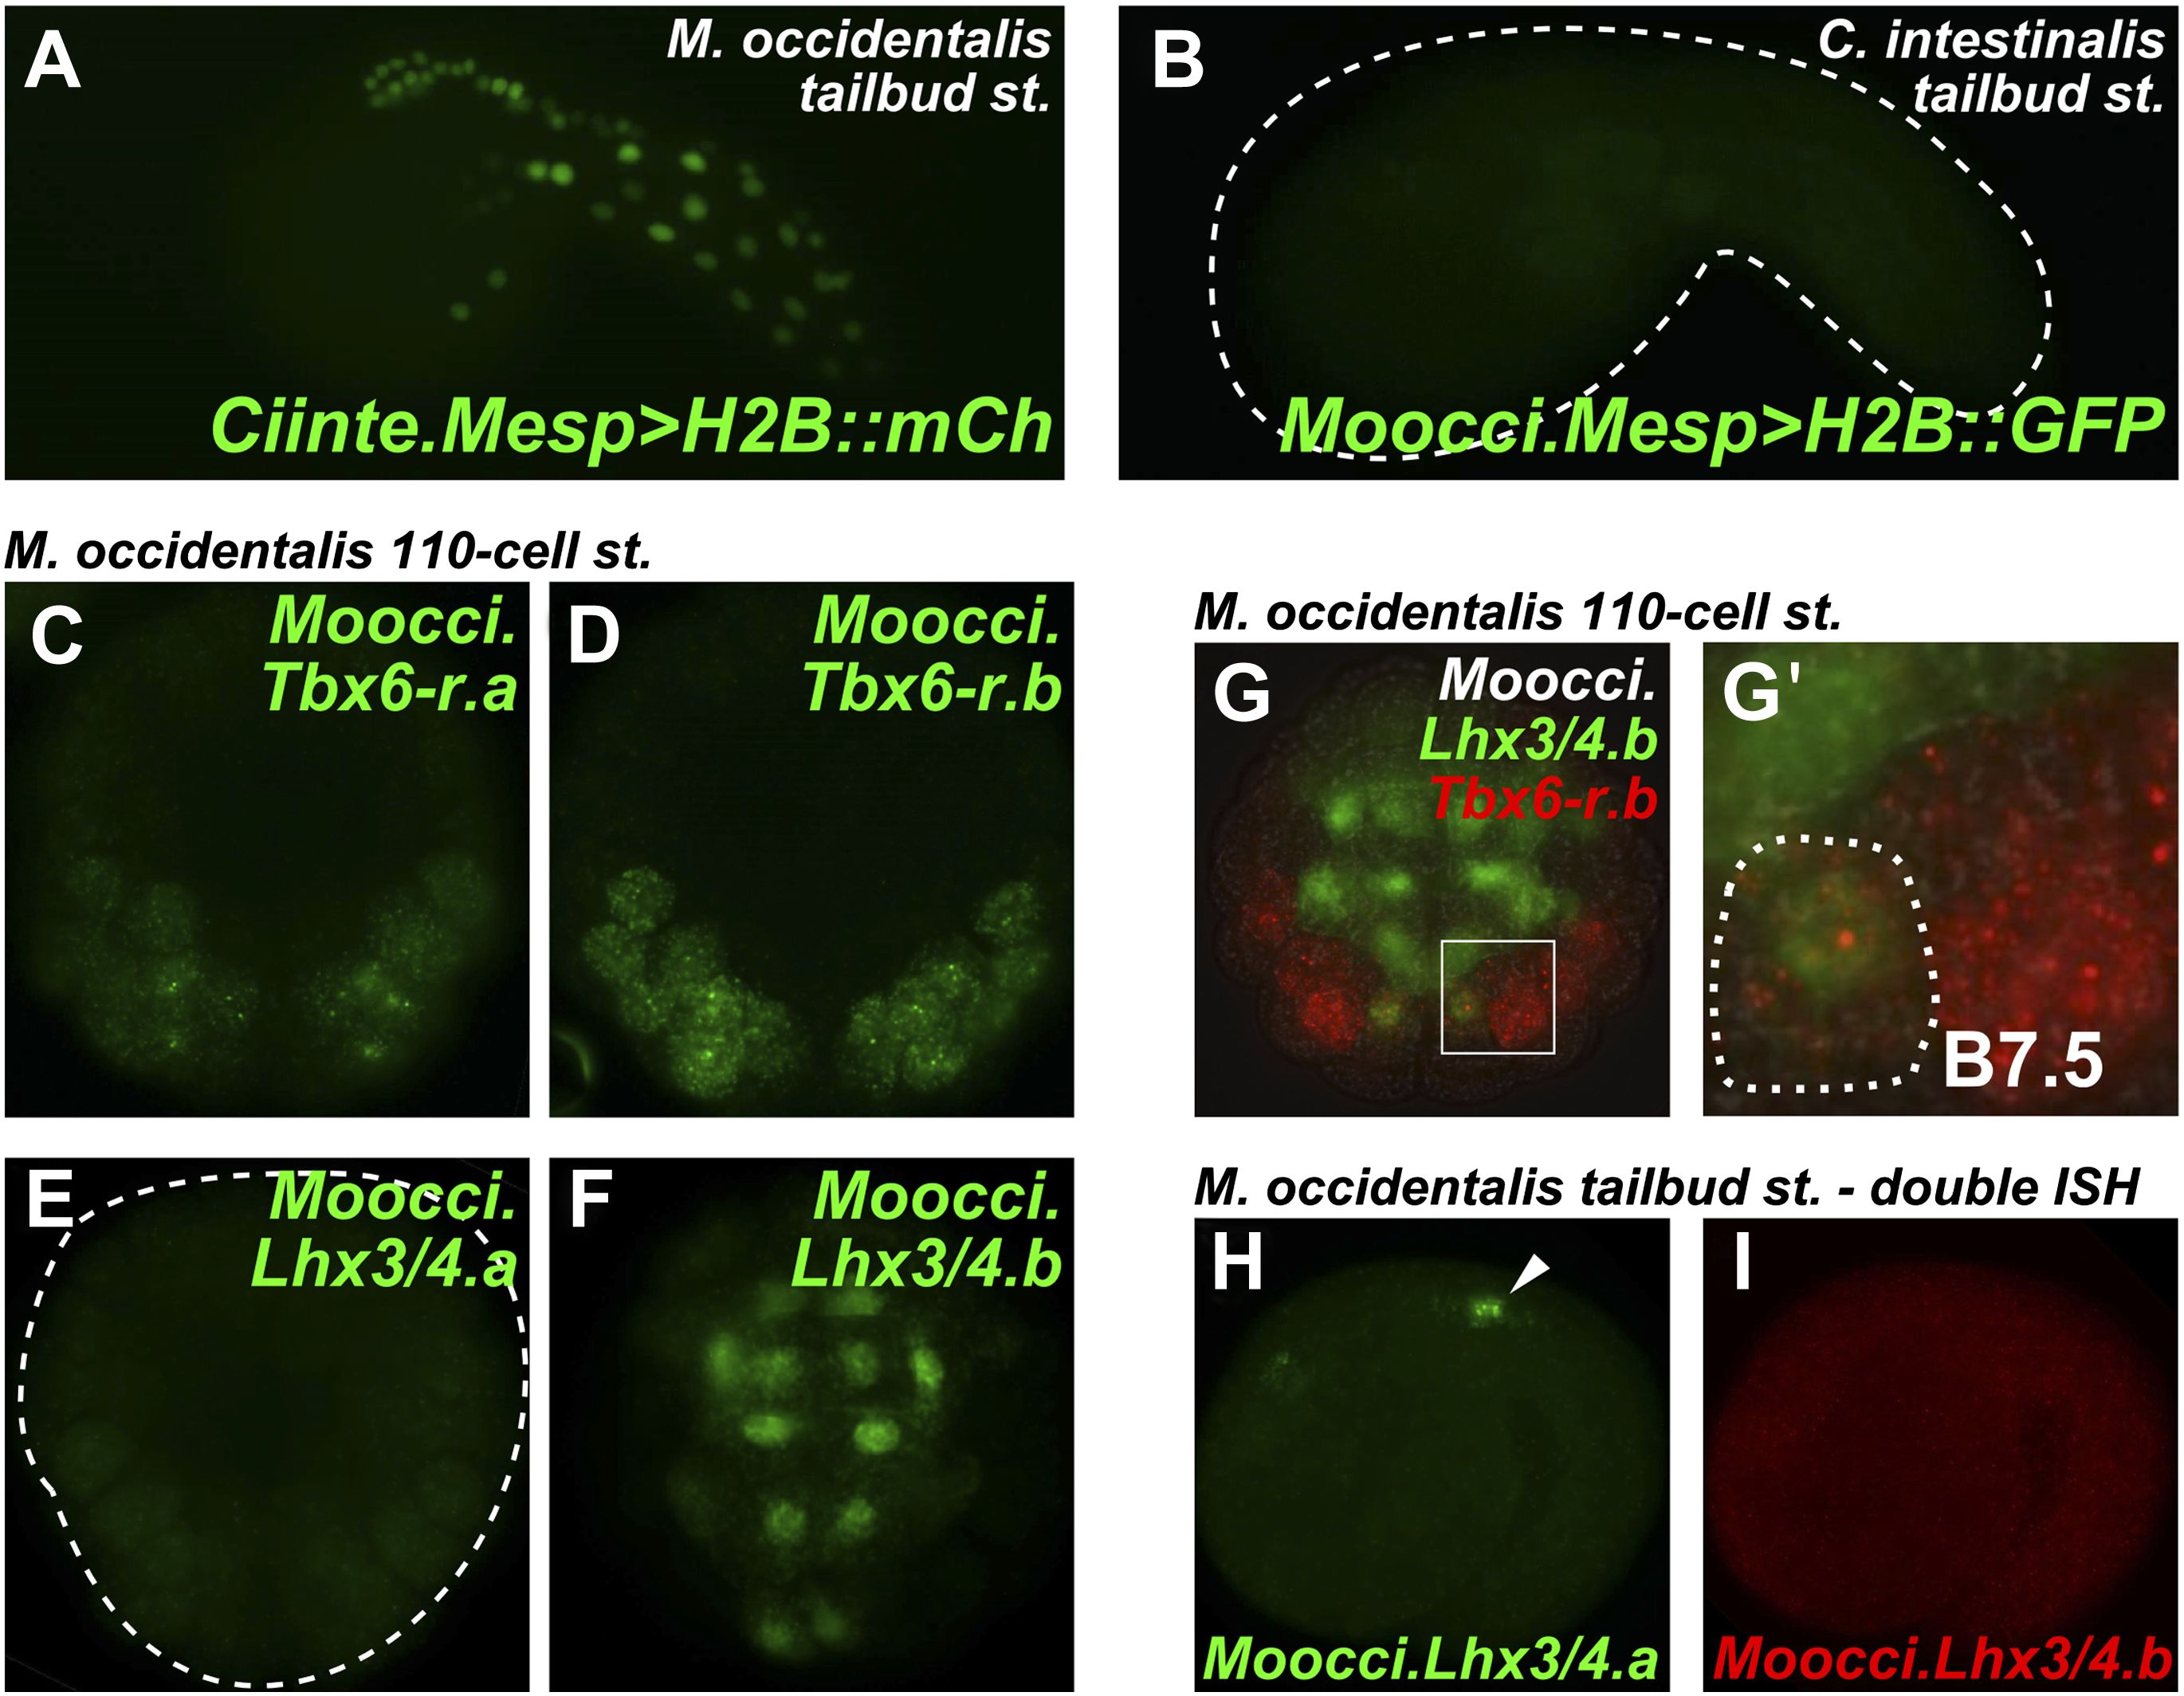
\includegraphics[scale=0.6]{figures/F14_large.jpg}
\caption{\textbf{The B7.5 lineage in \textit{M. occidentalis}}Cross-species reporter construct assays reveal multiple cases of cis-regulatory unintelligibility. (A) C. intestinalis embryo electroporated with Ciinte.Tbx6-r.b>GFP reporter construct (Christiaen et al., 2009a), which drives GFP expression in tail muscles and the B7.5 lineage cells (arrowheads), recapitulating endogenous Ciinte.Tbx6-r.b expression. (B) M. occidentalis embryo electroporated with Moocci.Tbx6-r.b$>$GFP reporter construct, which recapitulates expression in tail muscle cells including B7.5 lineage cells (arrowheads). (C) C. intestinalis embryo electroporated with Moocci.Tbx6-r.b$>$GFP, which drives expression in B-line tail muscle and mesenchyme cells but is excluded from the B7.5 lineage. (D) C. intestinalis embryo electroporated with Ciinte.Hand-r$>$H2B::GFP reporter (Davidson and Levine, 2003), which drives H2B::GFP expression in anterior endoderm, A7.6 lineage, and TVCs (arrowheads), recapitulating endogenous Ciinte.Hand-r expression. (E) M. occidentalis embryo electroporated with Moccci.Hand-r>H2B::GFP construct, which recapitulates the same expression pattern. (F) C. intestinalis embryo electroporated with Moocci.Hand-r$>$H2B::GFP, which drives expression in endoderm and A7.6 lineage, but not in B7.5. (G) M. occidentalis embryo electroporated with Ciinte.Ebf neuron-specific YFP (green) and H2B::mCherry (red) reporter constructs electroporated (Stolfi and Levine, 2011), which drive very weak expression in a limited subset of motor ganglion neurons (green and red). (H) C. intestinalis embryo electroporated with a Moocci.Ebf$>$YFP reporter, which drives robust reporter gene expression in several brain, motor ganglion, and nerve cord neurons. (I) C. intestinalis embryos electroporated with Ciinte.Sox1/2/3 (left) and Moocci.Sox1/2/3 (right) H2B::mCherry reporter constructs, both of which recapitulate Sox1/2/3 expression in ectoderm. Panels A?F are lateral views of tailbud embryos, panels G is a dorsal view of a tailbud embryo, panel H is a dorso-lateral view of a hatched larva, and panel I shows vegetal views of mid-gastrula stage embryos. Anterior is to the right, except in Panel I, in which anterior is to the top. DOI: 10.7554/eLife.03728.023}
\label{fig:tbx}
\end{figure}

\section{Discussion}
Three \textit{Molgula}\textemdash\textit{M. occulta}, \textit{M. oculata} and \textit{M. occidentalis}\textemdash species have been sequenced and assembled; these are the first of any molgulids to have assembled genomes. Developmentally the three species are very similar up to the gastrula stage, where \textit{M. occulta} diverge from the typical solitary ascidian body plan and develops without a tail \cite{berrill_studies_1931,nishida_cell_1987}. 

In vertebrate and other bilaterians the \textit{hox} genes has been shown to be important for patterning along the anterior-posterior axis \cite{finnerty_origins_2003,mallo_regulation_2013}. The same has not be shown in ascidians, where \textit{hox} has more of a tissue specific role \cite{ikuta_limited_2010}.  \textit{Ciona} has 10 \textit{hox} genes and is missing \textit{hox7-9} and \textit{11}, with \textit{hox10} and \textit{12} being the only two genes to show morphological effects when knocked down. \textit{Hox10} is involved in the regulation of the motor neuron differentiation and \textit{hox12} is involved in tail development, through the elongation of the posterior most section of the tail and of the epidermal cells at the tail tip \cite{ikuta_limited_2010}. We observed the absence of \textit{hox6} in all three \textit{Molgula} species, which is not surprising, seeing that \textit{hox6} is also missing in \textit{O. dioica} and no expression is detected in \textit{C. intestinalis} through whole mount in situ hybridization at any stage of development \cite{ikuta_ciona_2004,seo_hox_2004}. No two of the \textit{Molgula} species show the same \textit{hox} cluster and all show a strong divergence outside of coding regions, even more so in \textit{M. occidentalis}. There is a duplicate in \textit{M. occidentalis hox10} which could lead to a split in function since \textit{Ciona Hox10}  is expressed in two region during the mid-tailbud stage\textemdash a small region of the anterior nerve cord, and a small area of the posterior ventral endoderm and adjacent tissue \cite{ikuta_ciona_2004}. It is proposed that ascidians evolved their simple body plans and rapid embryogenesis through extensive genomic rearrangement and gene loss, with specific loss of several \textit{hox} genes \cite{ikuta_organization_2005}. \textit{Hox12-13} are not found on the same contig in \textit{M. occulta}, however when aligned with mVista there appears to be a strong case for synteny (Figure~\ref{fig:hox12}), so it is possible they are clustered, but the contigs are not joined because the \textit{M. occulta} genome assembly is too fragmented. \textit{Hox} function does not have the same level and so far their has not been a consistence between \textit{hox} clusters in no Tunicate studied, showing that \textit{hox} is tends do be divergent within the tunicates.

In \textit{Ciona} \textit{dll} stains in the endodermal strand cell during early-tailbud embryos, showing positive signals in two cells of the endodermal strand \cite{caracciolo_identification_2000} which derives from the primary muscle or mesenchyme lineage \cite{rossomando_morphogenesis:_1992}, while in Drosophila embryos \textit{dll} is required for the gene pathway for limb formation in the thoracic segment \cite{vachon_homeotic_1992}.Because of the lack of homology outside of coding regions, we were able to identify \textit{distal-less} (\textit{dll}) downstream of \textit{hox13} in both \textit{M. occidentalis} and \textit{M. oculata}, but we did not find it in \textit{M. occulta}.  Further investigation is needed, as this could potentially be tied to failed muscle cell differentiation in \textit{M. occulta}.

From our initial survey of a handful of enhancers from C. intestinalis, M. occidentalis, and M. oculata, we
encountered several instances of either mutual unintelligibility, or asymmetric intelligibility of enhancers. These results add to the mounting evidence suggesting that acute and pervasive DSD may
have occurred over the course of ascidian evolution, obfuscated by the identical cell lineages and
highly conserved gene expression patterns of ascidian embryos (Swalla, 2004). The multiple examples
of cis-regulatory unintelligibility we identified were rather unexpected given (a) the extremely conserved
pattern of expression of orthologous genes from Molgula and Ciona (Takada et al., 2002) and
(b) previous observations of mutual intelligibility of enhancers between C. intestinalis and H. roretzi
(e.g., Otx), and between C. intestinalis and the more closely related C. savignyi (Johnson et al., 2004;
Brown et al., 2007). Large-scale, quantitative cross-species assays and detailed GRN studies will
illuminate factors that may contribute to conservation or divergence in regulatory mechanisms.

\section{Conclusion}
\textit{Hox} genes function is not conserved within the tunicates, which have also undergone substantial \textit{hox} gene loss. All central \textit{hox} genes are missing in all three \textit{Molgula} species. Studying these three molgula species have compounded the evidence that Tunicate has loss both \textit{hox7} and \textit{hox8} after diverging from the vertebrates and cephalochordates, while ascidians have lose \textit{hox9} and \textit{hox11} after diverging from the larvaceans. It appears because \textit{hox} does not act as in the same role as anterior-posterior organizer, \textit{hox} genes are more easily lost in ascidians and other genes have taking over this role. 

Although tunicates have a well defined and invariant cleavage, the mechanism behind development is not always the same from species to species.% We have demonstrated that tunicates with the same different \textit{M. occidentalis} has shown. 
We speculate that a high frequency of compensatory changes, required for the rapidly evolving
ascidians to accommodate the constraints imposed by their invariant embryonic cell lineages and
highly compact genomes, has given rise to a preponderance of cross-species cis-regulatory unintelligibility,
following the DSD/SPC model. This perfect storm of intrinsic factors may be the key to
explaining the dichotomy observed between highly conserved embryos and divergent cis-regulatory
structure/function in ascidians.
